\section{Offline RL: Advancements and Challenges}

\textbf{Offline Reinforcement Learning} (RL)
has emerged as a promising approach for training control
policies using pre-collected experiences,
eliminating the need for potentially dangerous or
costly online interactions. Despite significant progress
in this field, several challenges persist in
its practical application, particularly in control
and robotics domains.

Research efforts to enhance Offline RL performance are
primarily advancing along two paths.

\subsection{Improving Robustness and Sample Efficiency}

The first research direction focuses on refining
existing methods to enhance their robustness and
sample efficiency. \cite{kumar2021} propose a comprehensive
workflow for offline model-free robotic reinforcement
learning. Their approach addresses challenges specific
to real-world robotics applications, proposing
metrics and protocols to assist practitioners in
selecting policy checkpoints, regularization parameters,
and model architecture.

\cite{ijcai2023} introduce a hierarchical approach called
``Guide to Control'' that solves efficiently long-horizon
and sparse-reward tasks from offline data.
This method enhances the effectiveness
of offline RL in complex environments by breaking down the overall
task into more manageable sub-tasks, thereby improving learning
efficiency and performance.

\subsection{Developing Datasets and Benchmarks}

The second path concentrates on creating extensive datasets
and benchmarks tailored for control and robotics domains.
\cite{gurtler2023} present a benchmark for offline RL
on real-robot hardware, providing a crucial resource for
evaluating algorithms in practical settings.
In their work they propose a set of
benchmark datasets for robotic manipulation
that are intended to help improving the
state-of-the-art in offline reinforcement learning.

\cite{liu2023} contribute datasets and benchmarks
specifically designed for offline safe reinforcement learning
to accelerate research in this area.
Their work addresses the critical aspect of safety in robotic
applications, providing resources for researchers to develop and
test algorithms that not only optimize performance but also ensure
safe operation in various scenarios. The suite comprises three
main components: expertly crafted safe policies, D4RL-styled
datasets with environment wrappers, and high-quality offline
safe RL baseline implementations. The authors present a methodical
data collection pipeline using advanced safe RL algorithms to generate
diverse datasets across 38 popular safe RL tasks,
ranging from robot control to autonomous driving.
They also introduce data post-processing filters to
modify dataset diversity, simulating various data collection conditions.

\section{Data Augmentation Strategies in RL}

Despite ongoing improvements in learning algorithms,
the quantity of training data continues to be a critical
determinant of success in machine learning processes.
This is especially challenging when dealing with complex,
high-dimensional inputs such as images, where the data requirements
for effective training are substantial.

To address the problem of limited data availability,
researchers and practitioners often turn to
\textbf{data augmentation techniques}.
These methods aim to expand existing datasets by generating
synthetic samples that are both artificial and plausible,
thereby enriching the training set without the need
for additional real-world data collection.

\cite{mumini2022} provide a comprehensive survey of modern data
augmentation approaches, highlighting their potential in
enhancing computer vision across various domains.

\subsection{Augmentation in Online and Offline RL}

Both online and offline RL approaches have incorporated data
augmentation techniques to improve learning efficiency and generalization.

In the \textbf{online} RL setting, \cite{laskin2020}
introduce Reinforcement Learning with Augmented Data (RAD), 
a simple module designed to enhance most RL algorithms.
The authors conduct an extensive study of various data augmentation
techniques for both pixel-based and state-based inputs in RL, including
two new augmentations they introduce: random translate and random
amplitude scale.

\cite{hansen2021} further further explore the concept of data augmentation
in online RL, proposing SOft Data Augmentation (SODA),
a novel approach to improve generalization in RL;
unlike traditional methods that directly learn policies
from augmented data, SODA decouples augmentation from policy learning.
It does this by applying a soft constraint on the encoder to
maximize mutual information between latent representations of
augmented and non-augmented data, while using only non-augmented
data for RL optimization.

In the \textbf{offline} RL setting, \cite{han2022}
introduce a selective data augmentation technique
using a Variational Autoencoder (VAE).
The method targets sparse subspaces in the dataset,
representing them in the VAE's latent space,
then sampling and decoding new data points to augment
underrepresented regions. This approach aims to generate
virtual data that closely aligns with the original data distribution.

\cite{joo2022} propose a data augmentation method for offline RL
called Swapping Target Q-Value (SQV).
SQV works by swapping Q-values between original and transformed images,
encouraging the algorithm to treat similar states as equivalent while
emphasizing differences between distinct states.
This method aims to enhance pixel-based learning without auxiliary
loss functions, potentially improving performance and generalization
in offline RL scenarios with limited datasets.

\subsection{Dynamics-Aware Augmentation}

Traditional augmentation methods often operate without
knowledge of the underlying environment dynamics, requiring
careful tuning to avoid generating inconsistent samples.
To mitigate this issue, dynamics-aware augmentation schemes
have emerged in the robotics field.

In a paper by \cite{lin2020} the authors introduce a
framework called
\textbf{Invariant Transform Experience Replay}
to improve Deep Reinforcement Learning (DRL)
for robot control.
The main idea is to use symmetries in robotic
tasks to create more training data by exploiting
reflectional symmetries and taking advantage of
flexible goal definitions.

Nonetheless, effectively implementing these techniques
requires an in-depth understanding
of the underlying process, which is often not available, and
the development of an augmentation strategy specifically
crafted for the task at hand.

\section{Learning-Based Approaches to Data Generation}

Researchers are increasingly turning to data-driven methods
to overcome these obstacles. These approaches aim to learn
the underlying data generation model from the offline
dataset itself. After the model is trained,
it can be used to produce new samples that align
with the environment's dynamics. This strategy allows
for the creation of synthetic data that is more likely
to be consistent with the real-world processes
being modeled, without requiring explicit knowledge
of those processes.

\subsection{Transformer-Based Models}

\cite{wang2022} introduce the Bootstrapped Transformer,
a novel algorithm for offline RL.
They approach offline RL as a sequence generation
problem, using \textbf{Transformer} models to represent
trajectories. Recognizing the common issue of
limited and insufficiently diverse training
data in offline RL datasets, they implement a
\textbf{bootstrapping technique}: 
this allows the model to generate additional
offline data using its own learned representations,
which is then used to enhance the training of
the sequence model.

\subsection{World Models and Variational Autoencoders}

\textbf{World Models}, introduced in \cite{ha2018},
are a class of models that combine a Variational
Autoencoder as a Vision module,
a Recurrent Neural Network (RNN)
with a Mixture Density Network (MDN) as a Memory
module and a simple Neural Network (NN)
layer as a Controller.
These models can be trained
quickly in an unsupervised manner to learn a
compressed spatial and temporal representation
of the environment.

A Variational Autoencoder (VAE),
defined in \cite{kingma2013},
is an unsupervised learning architecture
that learns a low-dimensional latent space
representation of the input data
by encoding and decoding it through
two separate neural networks.
\label{sec:vae}

Despite not being explicitly designed for data augmentation,
World Models and VAEs
can be naturally used to achieve the same objective.

\cite{hafner2020} 
introduces \textbf{Dreamer}, a reinforcement learning
agent that uses a learned world model to solve complex
tasks from visual inputs. Dreamer learns a compact
latent space representation of the environment and
uses this model to imagine trajectories and learn
behaviors through ``latent imagination''.
The agent learns both actions and state values in the
latent space, efficiently optimizing behavior
by propagating analytic gradients of learned
state values through imagined trajectories.

A similar approach was proposed in \cite{andersen2018}
where the \textbf{Dreaming Variational Autoencoder} (DVAE)
architecture is presented.
The DVAE combines variational autoencoders
with deep reinforcement learning agents,
allowing agents to learn optimal policies using
generated training data samples. To test this approach,
the authors also present \textbf{Deep Maze}, a novel and flexible
maze engine that provides various challenges
for reinforcement learning algorithms,
including partial and fully-observable state-spaces,
long-horizon tasks, and both deterministic and
stochastic problems.

\section{Counterfactual Reasoning in Data Generation}

The \textbf{counterfactual-based approach} offers a
versatile and robust alternative rooted in
the theory of \textbf{Structural Causal Models} (SCMs) 
(which are discussed in more detail in Section
\ref{sec:scm}).
This method begins by modeling the system's
dynamics using an SCM, which is then employed
for counterfactual reasoning. This process generates
new samples as counterfactual outcomes that align with
the model. Unlike previous methods, SCMs provide
tools to model and estimate unmeasured variables,
enabling a more precise depiction of the factors
affecting the system's behavior.

\subsection{Counterfactual Generative Models}

\cite{sauer2021} introduce the
\textbf{Counterfactual Generative Network} (CGN),
a novel approach to improve the robustness and
interpretability of image classifiers.
The authors propose decomposing the image
generation process into independent causal
mechanisms that disentangle object shape, texture
and background. This allows for the generation of
counterfactual images, synthetic images with novel
combinations of these features.
The CGN is trained without direct supervision,
using only class labels and inductive biases and
the authors demonstrate the CGN's ability to
generate counterfactual images
on MNIST and ImageNet datasets, as shown
in Figure \ref{fig:ctf}.

\begin{figure}[ht]
    \centering
    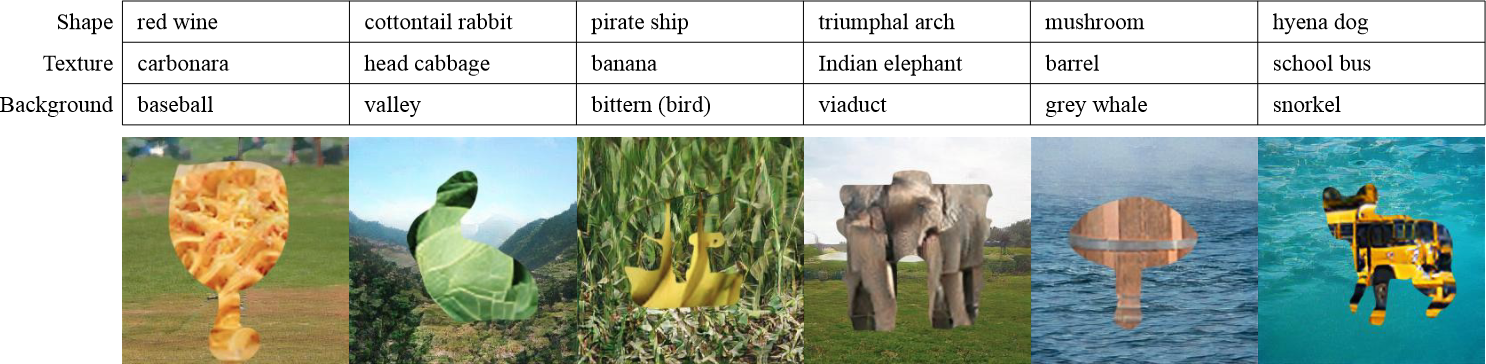
\includegraphics[width=\textwidth]{figures/ch2/1.ctf.png}
    \caption{ImageNet Counterfactuals produced by the CGN}
    \vspace{-10px}
    \caption*{\scriptsize{Source: \cite{sauer2021}}}
    \label{fig:ctf}
\end{figure}

Another usage of counterfactual reasoning,
this time in the context of medical imaging,
is presented in \cite{mertes2022}.
This paper introduces GANterfactual,
a novel approach for generating counterfactual
explanations for image classifiers using adversarial
image-to-image translation techniques.
Unlike traditional methods that highlight
important areas in images, GANterfactual
modifies input images to change the
classifier's prediction,
providing users with a different kind
of explanatory information.
The authors focus on medical contexts,
specifically pneumonia detection in chest X-rays,
where textural and structural information is crucial.

\subsection{Counterfactual Data Augmentation in Offline RL}

\cite{lu2020} investigate counterfactual-based
data augmentation
specifically in the context of Offline RL.
They propose a Deep Generative Model based on the
Bidirectional Conditional Generative Adversarial Network
(BiCoGAN) architecture (which is discussed in more detail
in Section \ref{sec:bicogan}), the model
can be seen in Figure \ref{fig:rlcf}.
The authors use structural causal models (SCMs)
to model state dynamics, leveraging both
commonalities and differences across subjects,
and allowing to estimate unmeasured variables,
which are then used to effectively
reproduce the environment’s initial conditions
and enable the
generation of counterfactual outcome.
They prove that counterfactual outcomes are identifiable
under mild conditions and that a Double Dueling
Deep Q-Network (discussed in Section \ref{sec:rl})
trained on both the augmented dataset and the original
counterpart achieves better performance on the first one.

\begin{figure}[h]
    \centering
    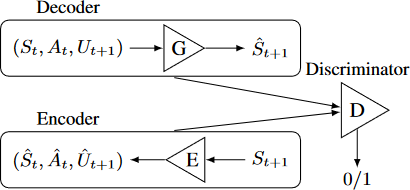
\includegraphics[width=.5\textwidth]{figures/ch2/2.rlcf.png}
    \caption{The proposed Deep Generative Model for Counterfactual Data Augmentation in Offline RL}
    \vspace{-10px}
    \caption*{\scriptsize{Source: \cite{lu2020}}}
    \label{fig:rlcf}
\end{figure}

However, this approach is designed for non-visual,
low-dimensional inputs, and discrete control
actions. Additionally, a significant drawback of this algo-
rithm is its lack of a mechanism for estimating the reward
associated with the generated states. This limitation implies
that retrieving the reward is possible only when the reward
function can be directly calculated from the generated states,
a condition that does not always apply.


